\documentclass[a4paper,10pt]{article}
\usepackage[utf8]{inputenc}
\usepackage[T1]{fontenc}
\usepackage[english]{babel}
\usepackage[a4paper,top=2.5cm, bottom=2.5cm, left=2.5cm, right=2.5cm]{geometry}
\usepackage{graphicx}

\title{Software Architectures\\ Assignment 2 : Architectural Patterns}
\author{Arnaud Rosette, Simon Picard}

\begin{document}
\maketitle

\section{Design flaws discovered in the implementation of the three-tier architecture}
\subsection{Where did you need to change another layer in order to get your new implementation to work ?}
One problem in the initial implementation of the three-tier architecture is that the two layers on top of the database layer have to know how the database layer works internally because the InternetFrontEnd (ui layer) and ApplicationFacade (application layer) classes knew that the initially used sql database uses a username, password and url. So the problem with this implementation is that changing the database type implies modifying the three layers. \\
Our solution to fix this problem is passing an object of the Properties class (which contains the parameters from the configuration file) along the different layers. With this solution, each layer takes the informations it needs from the configuration file. 
\subsection{How did you improve the architecture to facilitate adding new implementation for a layer in the future ?}
The problem here is that each facade uses directly a concrete implementation of a layer. The solution we implemented for the database layer is the database facade communicate with interfaces and the creation of the concrete database is delegated to a factory which chooses which type of database has to be created according to the configuration file.\\
In order to improve the architecture to facilitate adding new implementation of a layer, the client classes (facade classes) have to interact with interfaces and the creation of the objects that compose a layer has to be delegated to another class (abstract factory pattern). With this solution adding a new implementation of a layer can be done only by adding new classes which implement these interfaces and creating a new concrete factory. The client code does not need to change which is easier for adding new implementations.

\subsection{Which changes would need to be done or have been done to achieve a clean separation between the layers? Clearly identify the problem, and describe how the code could be refactored.}
First of all, as mentionned above, the way configuration file is accessed has been changed in order to hide the implementation of the database layer from other layers.\\
Another problem is that the classes in the package data have methods such as asSql or asXml. So these classes know that they will be serialized in xml or sql and so these classes are aware of the underlying concrete database. A better idea is to let the underlying concrete database serialize the model objects itself.
\newpage
\section{Class diagram of the new database layer}
\begin{center}
\begin{figure}[h]
  \centerline{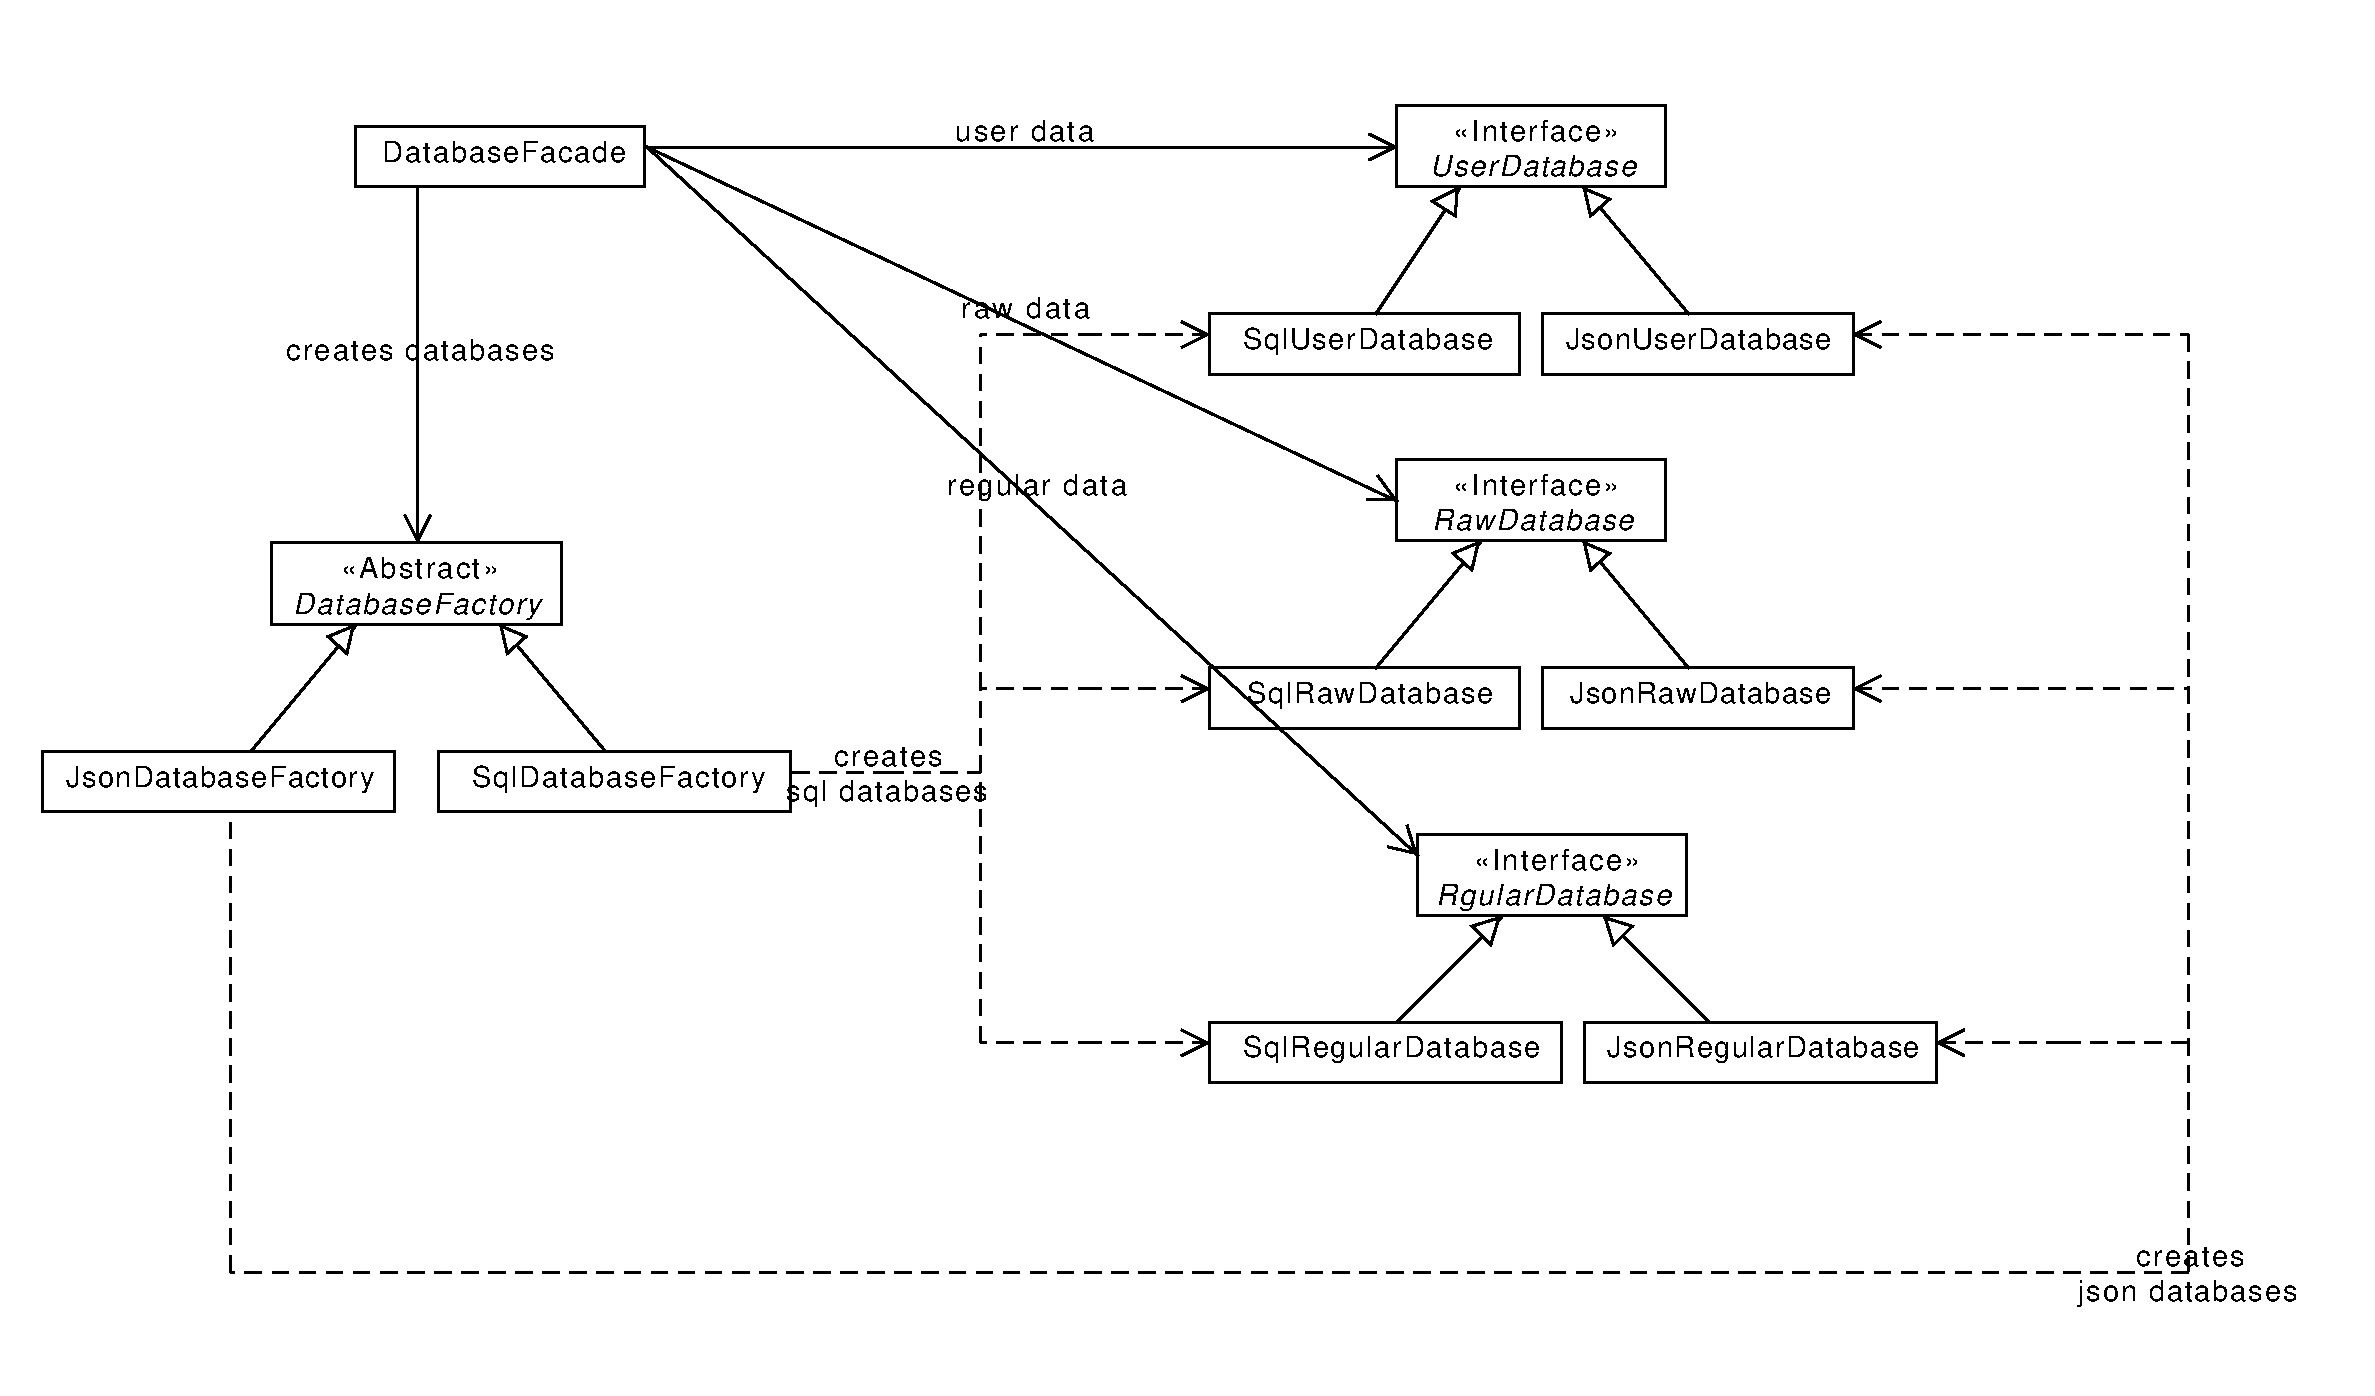
\includegraphics[width=0.9\textwidth]{class-diagram.pdf}}
  \caption{Database layer class diagram}
\end{figure}
\end{center}

\section{How switching between two implementations ?}
The configuration file contains 4 entries related to the database : dbUser (the username for the database), dbPassword (the password for the user specified previously), dbUrl (the location of the database) and dbType (the type of the database).\\
First of all, dbType may have two values : JSON or SQL.\\
If we want to use the sql database, we have to set the parameters the same way as before the modifications and the dbType parameter to SQL.
\begin{verbatim}
dbUser=SA
dbPassword=
dbUrl=file:/home/arnaud/Documents/ulb/ma1-2014-2015/MA1weekly/INFOY080/Project2/
      web_portal/DB/web_portal;ifexists=true;shutdown=true
dbType=SQL
\end{verbatim}
If we want to use the json database, we only have to set the dbUrl (location of the json file containing the database) and dbType parameters. For this implementation of the json database we choose to store all the database into one json file. If this file does not exist, it will be created.
\begin{verbatim}
dbUser=
dbPassword=
dbUrl=/home/arnaud/test.json
dbType=JSON
\end{verbatim}


\section{How does the facade pattern facilitate switching between different implementations of a layer ?}
Each layer communicates with the bottom layer by the intermediate of a facade class. So the only class exposed by a layer to the upper layer is the facade class. The facade classes are interfaces between each layer. They are contract between two layers. So the functionalities (methods) proposed by a facade should never change. The facade pattern helps hiding the internal behavior of a layer.\\
If we want to modify the internal behavior of a layer, we only have to conserve the interface proposed by its facade. We can modify anything else in the layer. So the facade pattern is here really useful and facilitate switching between different implementation of a layer.

\end{document}